\section{Ethereum and smart contracts}
\subsection{Smart Contracts and Ethereum}

\paragraph{Smart contract:}
\begin{itemize}
    \item computerized transaction protocol, that executes the terms of a contract.
    \item Minimizes the need for trusted intermediaries.
\end{itemize}{}

\paragraph{Ethereum:}
\begin{itemize}
    \item A decentralized platform designed to run smart contracts.
    \item Eth smart contracts are Turing-complete.
    \item Transactions change the state of one or more contracts.
    \item Latest block stores the latest local state of all smart contracts.
    \item Difference to Bitcoin:
    \begin{itemize}
        \item In Eth we own private keys to an account, not to a set of unspent transactions.
        \item In this account the balance is updated, we don't simply store unspent transactions.
        \item Account contains executable code.
    \end{itemize}{}
\end{itemize}{}

\paragraph{Ethereum accounts:}
\begin{itemize}
    \item \textbf{User accounts:} Owned by some person
    \begin{itemize}
        \item Can send transactions to transfer ether or trigger contract code.
        \item Contains Address and Ether balance.
    \end{itemize}
    \item \textbf{Contract accounts: } Owned by contract (autonomous).
    \begin{itemize}
        \item Code execution triggered by transactions that call functions.
        \item Contains Address, Ether balance, Associated contract code and persistent storage (state)
    \end{itemize}{}
\end{itemize}{}

\paragraph{Writing smart contracts:} Multiple high-level languages (Solidity, Vyper) and single low-level language (EVM bytecode). 

\begin{minipage}{0.75\linewidth}
    \centering      
    \def\svgwidth{\linewidth}
    %% Creator: Inkscape inkscape 0.92.4, www.inkscape.org
%% PDF/EPS/PS + LaTeX output extension by Johan Engelen, 2010
%% Accompanies image file 'L3_transactions.pdf' (pdf, eps, ps)
%%
%% To include the image in your LaTeX document, write
%%   \input{<filename>.pdf_tex}
%%  instead of
%%   \includegraphics{<filename>.pdf}
%% To scale the image, write
%%   \def\svgwidth{<desired width>}
%%   \input{<filename>.pdf_tex}
%%  instead of
%%   \includegraphics[width=<desired width>]{<filename>.pdf}
%%
%% Images with a different path to the parent latex file can
%% be accessed with the `import' package (which may need to be
%% installed) using
%%   \usepackage{import}
%% in the preamble, and then including the image with
%%   \import{<path to file>}{<filename>.pdf_tex}
%% Alternatively, one can specify
%%   \graphicspath{{<path to file>/}}
%% 
%% For more information, please see info/svg-inkscape on CTAN:
%%   http://tug.ctan.org/tex-archive/info/svg-inkscape
%%
\begingroup%
  \makeatletter%
  \providecommand\color[2][]{%
    \errmessage{(Inkscape) Color is used for the text in Inkscape, but the package 'color.sty' is not loaded}%
    \renewcommand\color[2][]{}%
  }%
  \providecommand\transparent[1]{%
    \errmessage{(Inkscape) Transparency is used (non-zero) for the text in Inkscape, but the package 'transparent.sty' is not loaded}%
    \renewcommand\transparent[1]{}%
  }%
  \providecommand\rotatebox[2]{#2}%
  \newcommand*\fsize{\dimexpr\f@size pt\relax}%
  \newcommand*\lineheight[1]{\fontsize{\fsize}{#1\fsize}\selectfont}%
  \ifx\svgwidth\undefined%
    \setlength{\unitlength}{720bp}%
    \ifx\svgscale\undefined%
      \relax%
    \else%
      \setlength{\unitlength}{\unitlength * \real{\svgscale}}%
    \fi%
  \else%
    \setlength{\unitlength}{\svgwidth}%
  \fi%
  \global\let\svgwidth\undefined%
  \global\let\svgscale\undefined%
  \makeatother%
  \begin{picture}(1,0.75)%
    \lineheight{1}%
    \setlength\tabcolsep{0pt}%
    \put(0,0){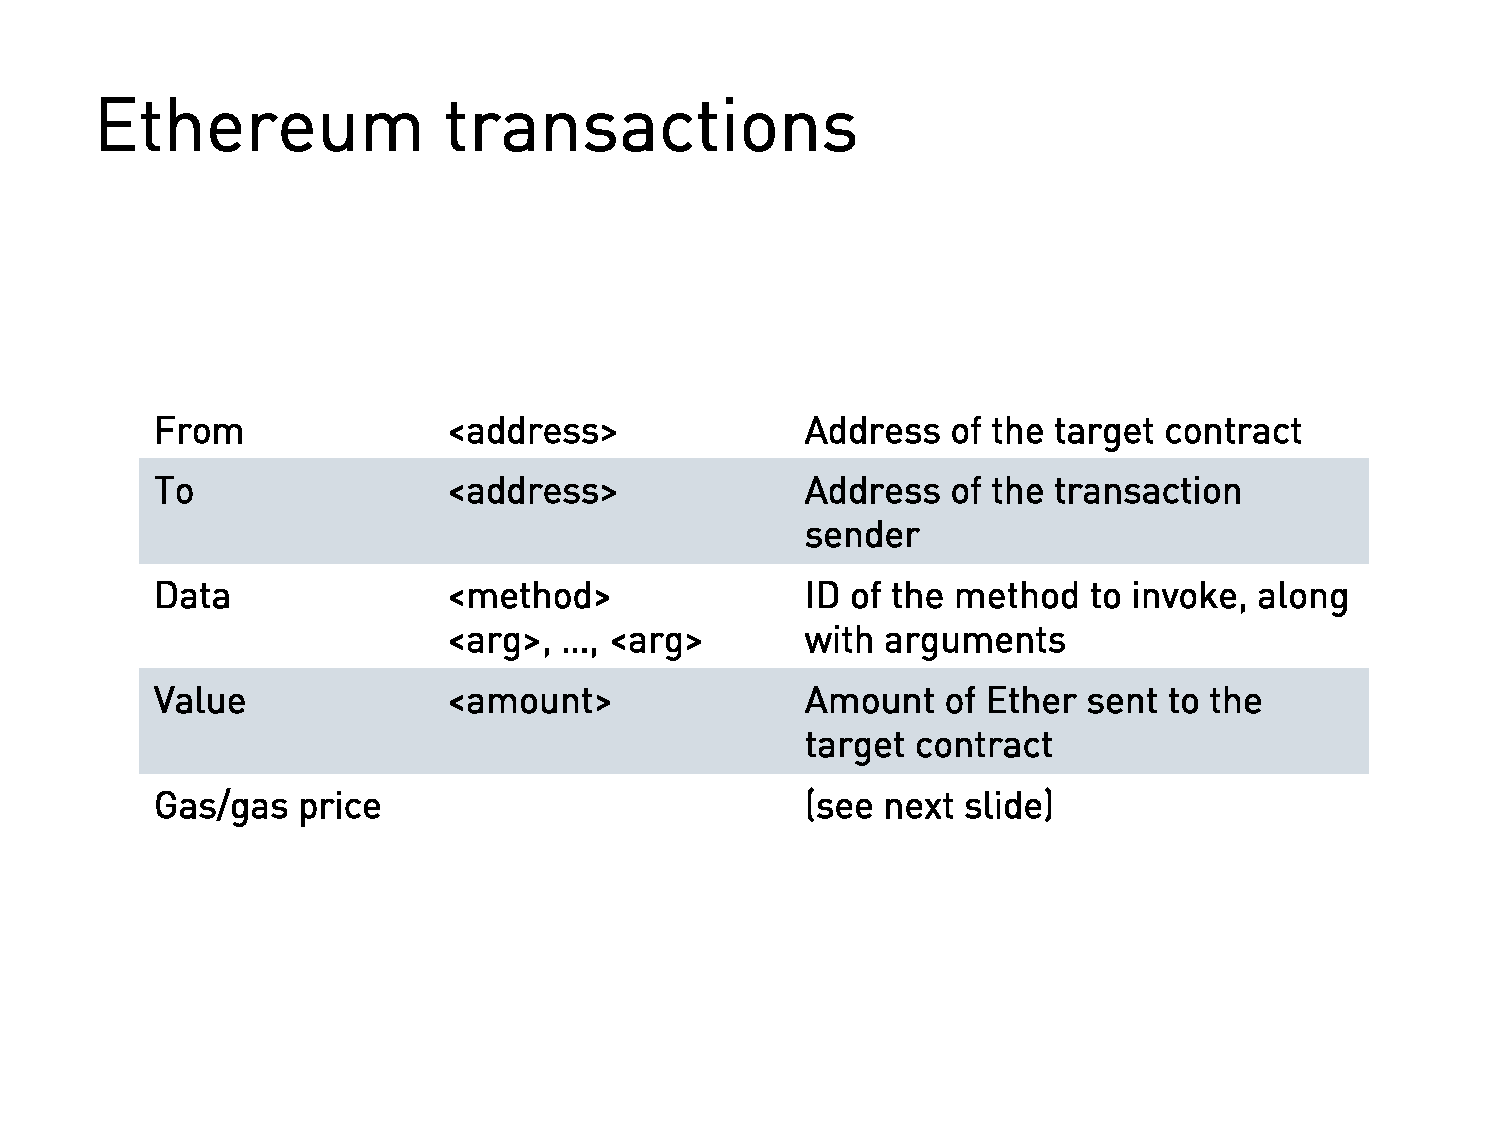
\includegraphics[width=\unitlength,page=1]{Figures/L3_transactions.pdf}}%
  \end{picture}%
\endgroup%



    
\end{minipage}

\paragraph{Gas: } How to prevent infinite loops in contract?
\begin{itemize}
    \item A transaction requires gas to fuel contract execution.
    \item Each EVM opcode has its amount of gas, it needs in order to be executed.
    \item Every transaction specifies a maximum amount of gas the sender is willing to spend.
    \item If the contract successfully executes, the unspent gas money is refunded to the sender.
    \item If execution runs out of gas, the execution is reverted, but gas money is not refunded.
    \item[\color{red}{$\xrightarrow{}$}] \textcolor{red}{Exploit:} The attacker can craft a transaction that triggers an out-of-gas exception at an arbitrary point in the execution. May create undesirable behaviors if not entire transaction is reverted.
\end{itemize}{}

\paragraph{Ether transfers:}
\begin{itemize}
    \item An ether transfer to a contract implicitly calls the receiver contract (called contract takes control over the execution).
    \item[\color{red}{$\xrightarrow{}$}] \textcolor{red}{Exploit:} Thus an attacker may own the external contract and execute arbitrary code. In particular, he can call back the contract before returning control to the caller.
    \item Any user can call arbitrary functions in contracts unless they have a \texttt{require(statement)} clause. This reverts the transaction if the statement is false
\end{itemize}{}

\begin{minipage}{0.75\linewidth}
    \centering      
    \def\svgwidth{\linewidth}
    %% Creator: Inkscape inkscape 0.92.4, www.inkscape.org
%% PDF/EPS/PS + LaTeX output extension by Johan Engelen, 2010
%% Accompanies image file 'ether_transfer_types.pdf' (pdf, eps, ps)
%%
%% To include the image in your LaTeX document, write
%%   \input{<filename>.pdf_tex}
%%  instead of
%%   \includegraphics{<filename>.pdf}
%% To scale the image, write
%%   \def\svgwidth{<desired width>}
%%   \input{<filename>.pdf_tex}
%%  instead of
%%   \includegraphics[width=<desired width>]{<filename>.pdf}
%%
%% Images with a different path to the parent latex file can
%% be accessed with the `import' package (which may need to be
%% installed) using
%%   \usepackage{import}
%% in the preamble, and then including the image with
%%   \import{<path to file>}{<filename>.pdf_tex}
%% Alternatively, one can specify
%%   \graphicspath{{<path to file>/}}
%% 
%% For more information, please see info/svg-inkscape on CTAN:
%%   http://tug.ctan.org/tex-archive/info/svg-inkscape
%%
\begingroup%
  \makeatletter%
  \providecommand\color[2][]{%
    \errmessage{(Inkscape) Color is used for the text in Inkscape, but the package 'color.sty' is not loaded}%
    \renewcommand\color[2][]{}%
  }%
  \providecommand\transparent[1]{%
    \errmessage{(Inkscape) Transparency is used (non-zero) for the text in Inkscape, but the package 'transparent.sty' is not loaded}%
    \renewcommand\transparent[1]{}%
  }%
  \providecommand\rotatebox[2]{#2}%
  \newcommand*\fsize{\dimexpr\f@size pt\relax}%
  \newcommand*\lineheight[1]{\fontsize{\fsize}{#1\fsize}\selectfont}%
  \ifx\svgwidth\undefined%
    \setlength{\unitlength}{730.7812546bp}%
    \ifx\svgscale\undefined%
      \relax%
    \else%
      \setlength{\unitlength}{\unitlength * \real{\svgscale}}%
    \fi%
  \else%
    \setlength{\unitlength}{\svgwidth}%
  \fi%
  \global\let\svgwidth\undefined%
  \global\let\svgscale\undefined%
  \makeatother%
  \begin{picture}(1,0.73893521)%
    \lineheight{1}%
    \setlength\tabcolsep{0pt}%
    \put(0,0){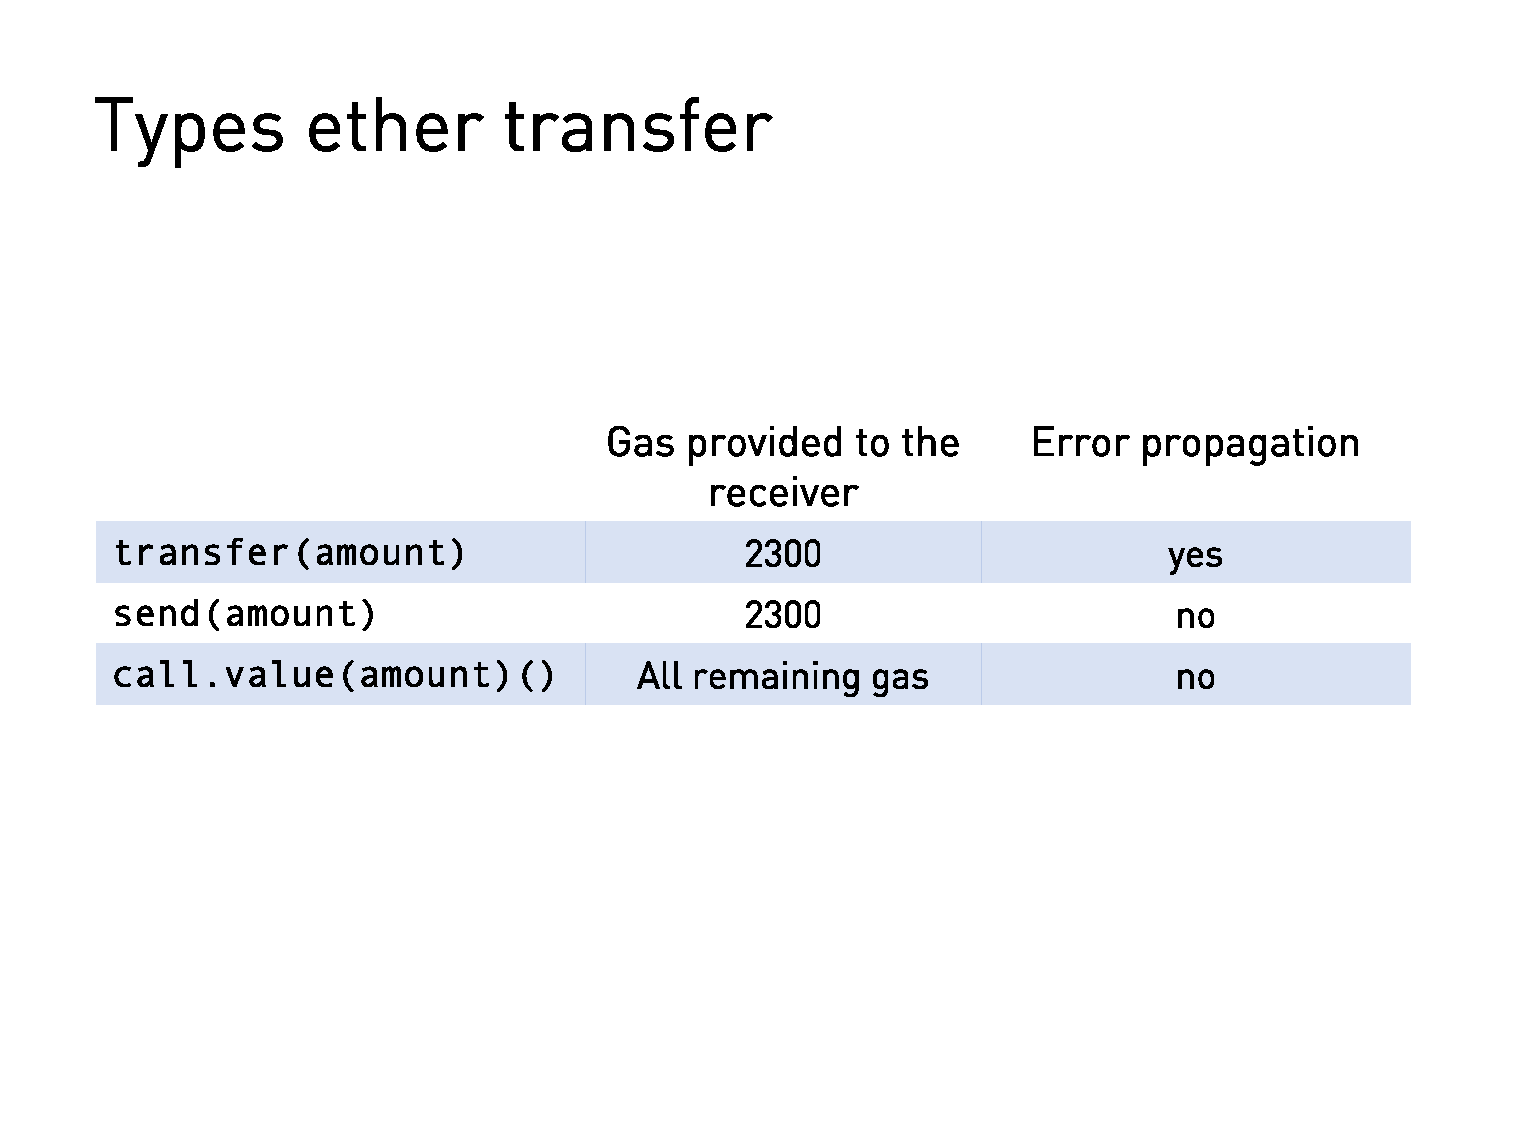
\includegraphics[width=\unitlength,page=1]{Figures/L3_ether_transfer_types.pdf}}%
  \end{picture}%
\endgroup%
    
\end{minipage}

\paragraph{Storage model} In the following variableID and mappingsId are just numbers that identify the variable (e.g. 0 for variable0, 1 for variable1, ..). 
\begin{itemize}
    \item \textbf{Variables:} value stored at \textcolor{blue}{offset} = $variableID$
    \item \textbf{Mappings:} mapping[key] stored at \textcolor{blue}{offset} = $SHA3(mappingID||key)$ 
    \item \textbf{Arrays:} array[10] stored at \textcolor{blue}{offset} = $SHA3(arrayID) + 10$
\end{itemize}{}

\subsection{Vulnerabilities of Smart Contracts}

\begin{enumerate}
    \item \textbf{The DAO bug:} Call \texttt{withdraw()} twice, first normally, then again before balance is set to zero.
    \item \textbf{BatchOverflow Exploit: }
\end{enumerate}{}

\begin{minipage}{0.45\linewidth}
    \centering      
    \def\svgwidth{\linewidth}
    %% Creator: Inkscape inkscape 0.92.4, www.inkscape.org
%% PDF/EPS/PS + LaTeX output extension by Johan Engelen, 2010
%% Accompanies image file 'L3_dao_bug.pdf' (pdf, eps, ps)
%%
%% To include the image in your LaTeX document, write
%%   \input{<filename>.pdf_tex}
%%  instead of
%%   \includegraphics{<filename>.pdf}
%% To scale the image, write
%%   \def\svgwidth{<desired width>}
%%   \input{<filename>.pdf_tex}
%%  instead of
%%   \includegraphics[width=<desired width>]{<filename>.pdf}
%%
%% Images with a different path to the parent latex file can
%% be accessed with the `import' package (which may need to be
%% installed) using
%%   \usepackage{import}
%% in the preamble, and then including the image with
%%   \import{<path to file>}{<filename>.pdf_tex}
%% Alternatively, one can specify
%%   \graphicspath{{<path to file>/}}
%% 
%% For more information, please see info/svg-inkscape on CTAN:
%%   http://tug.ctan.org/tex-archive/info/svg-inkscape
%%
\begingroup%
  \makeatletter%
  \providecommand\color[2][]{%
    \errmessage{(Inkscape) Color is used for the text in Inkscape, but the package 'color.sty' is not loaded}%
    \renewcommand\color[2][]{}%
  }%
  \providecommand\transparent[1]{%
    \errmessage{(Inkscape) Transparency is used (non-zero) for the text in Inkscape, but the package 'transparent.sty' is not loaded}%
    \renewcommand\transparent[1]{}%
  }%
  \providecommand\rotatebox[2]{#2}%
  \newcommand*\fsize{\dimexpr\f@size pt\relax}%
  \newcommand*\lineheight[1]{\fontsize{\fsize}{#1\fsize}\selectfont}%
  \ifx\svgwidth\undefined%
    \setlength{\unitlength}{720.00000454bp}%
    \ifx\svgscale\undefined%
      \relax%
    \else%
      \setlength{\unitlength}{\unitlength * \real{\svgscale}}%
    \fi%
  \else%
    \setlength{\unitlength}{\svgwidth}%
  \fi%
  \global\let\svgwidth\undefined%
  \global\let\svgscale\undefined%
  \makeatother%
  \begin{picture}(1,0.75)%
    \lineheight{1}%
    \setlength\tabcolsep{0pt}%
    \put(0,0){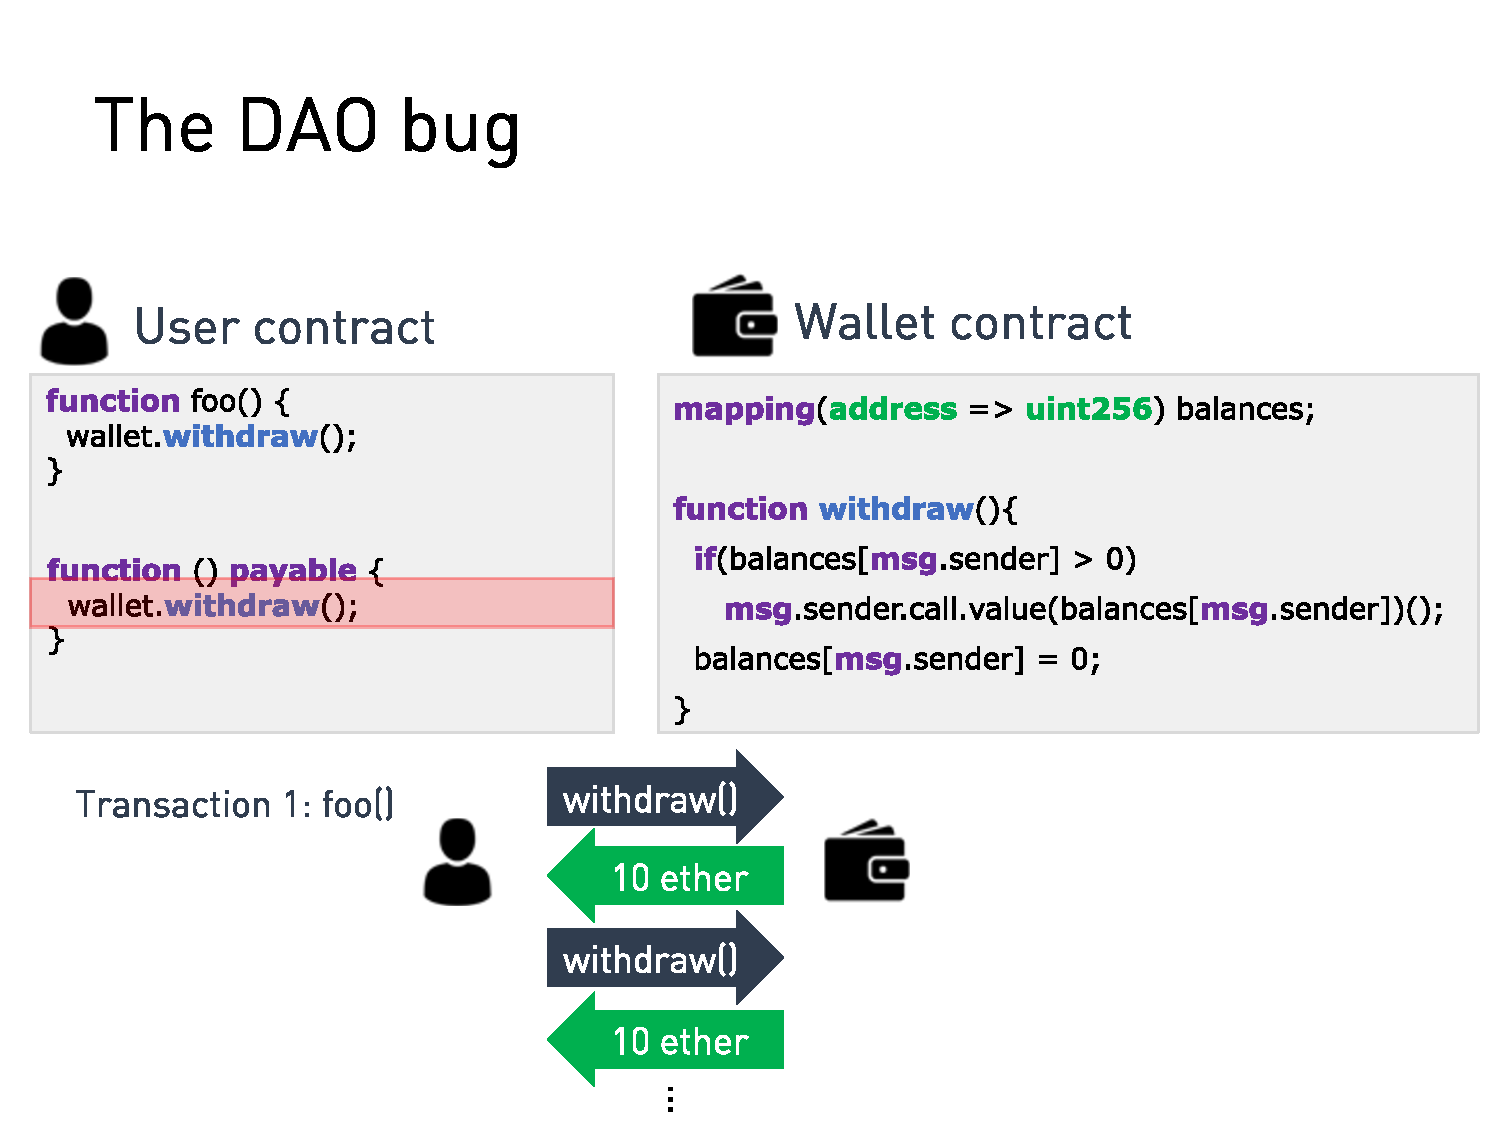
\includegraphics[width=\unitlength,page=1]{Figures/L3_dao_bug.pdf}}%
  \end{picture}%
\endgroup%
    
\end{minipage}
\begin{minipage}{0.45\linewidth}
    \centering      
    \def\svgwidth{\linewidth}
    %% Creator: Inkscape inkscape 0.92.4, www.inkscape.org
%% PDF/EPS/PS + LaTeX output extension by Johan Engelen, 2010
%% Accompanies image file 'L3_overflow_exploit.pdf' (pdf, eps, ps)
%%
%% To include the image in your LaTeX document, write
%%   \input{<filename>.pdf_tex}
%%  instead of
%%   \includegraphics{<filename>.pdf}
%% To scale the image, write
%%   \def\svgwidth{<desired width>}
%%   \input{<filename>.pdf_tex}
%%  instead of
%%   \includegraphics[width=<desired width>]{<filename>.pdf}
%%
%% Images with a different path to the parent latex file can
%% be accessed with the `import' package (which may need to be
%% installed) using
%%   \usepackage{import}
%% in the preamble, and then including the image with
%%   \import{<path to file>}{<filename>.pdf_tex}
%% Alternatively, one can specify
%%   \graphicspath{{<path to file>/}}
%% 
%% For more information, please see info/svg-inkscape on CTAN:
%%   http://tug.ctan.org/tex-archive/info/svg-inkscape
%%
\begingroup%
  \makeatletter%
  \providecommand\color[2][]{%
    \errmessage{(Inkscape) Color is used for the text in Inkscape, but the package 'color.sty' is not loaded}%
    \renewcommand\color[2][]{}%
  }%
  \providecommand\transparent[1]{%
    \errmessage{(Inkscape) Transparency is used (non-zero) for the text in Inkscape, but the package 'transparent.sty' is not loaded}%
    \renewcommand\transparent[1]{}%
  }%
  \providecommand\rotatebox[2]{#2}%
  \newcommand*\fsize{\dimexpr\f@size pt\relax}%
  \newcommand*\lineheight[1]{\fontsize{\fsize}{#1\fsize}\selectfont}%
  \ifx\svgwidth\undefined%
    \setlength{\unitlength}{720.00000454bp}%
    \ifx\svgscale\undefined%
      \relax%
    \else%
      \setlength{\unitlength}{\unitlength * \real{\svgscale}}%
    \fi%
  \else%
    \setlength{\unitlength}{\svgwidth}%
  \fi%
  \global\let\svgwidth\undefined%
  \global\let\svgscale\undefined%
  \makeatother%
  \begin{picture}(1,0.75)%
    \lineheight{1}%
    \setlength\tabcolsep{0pt}%
    \put(0,0){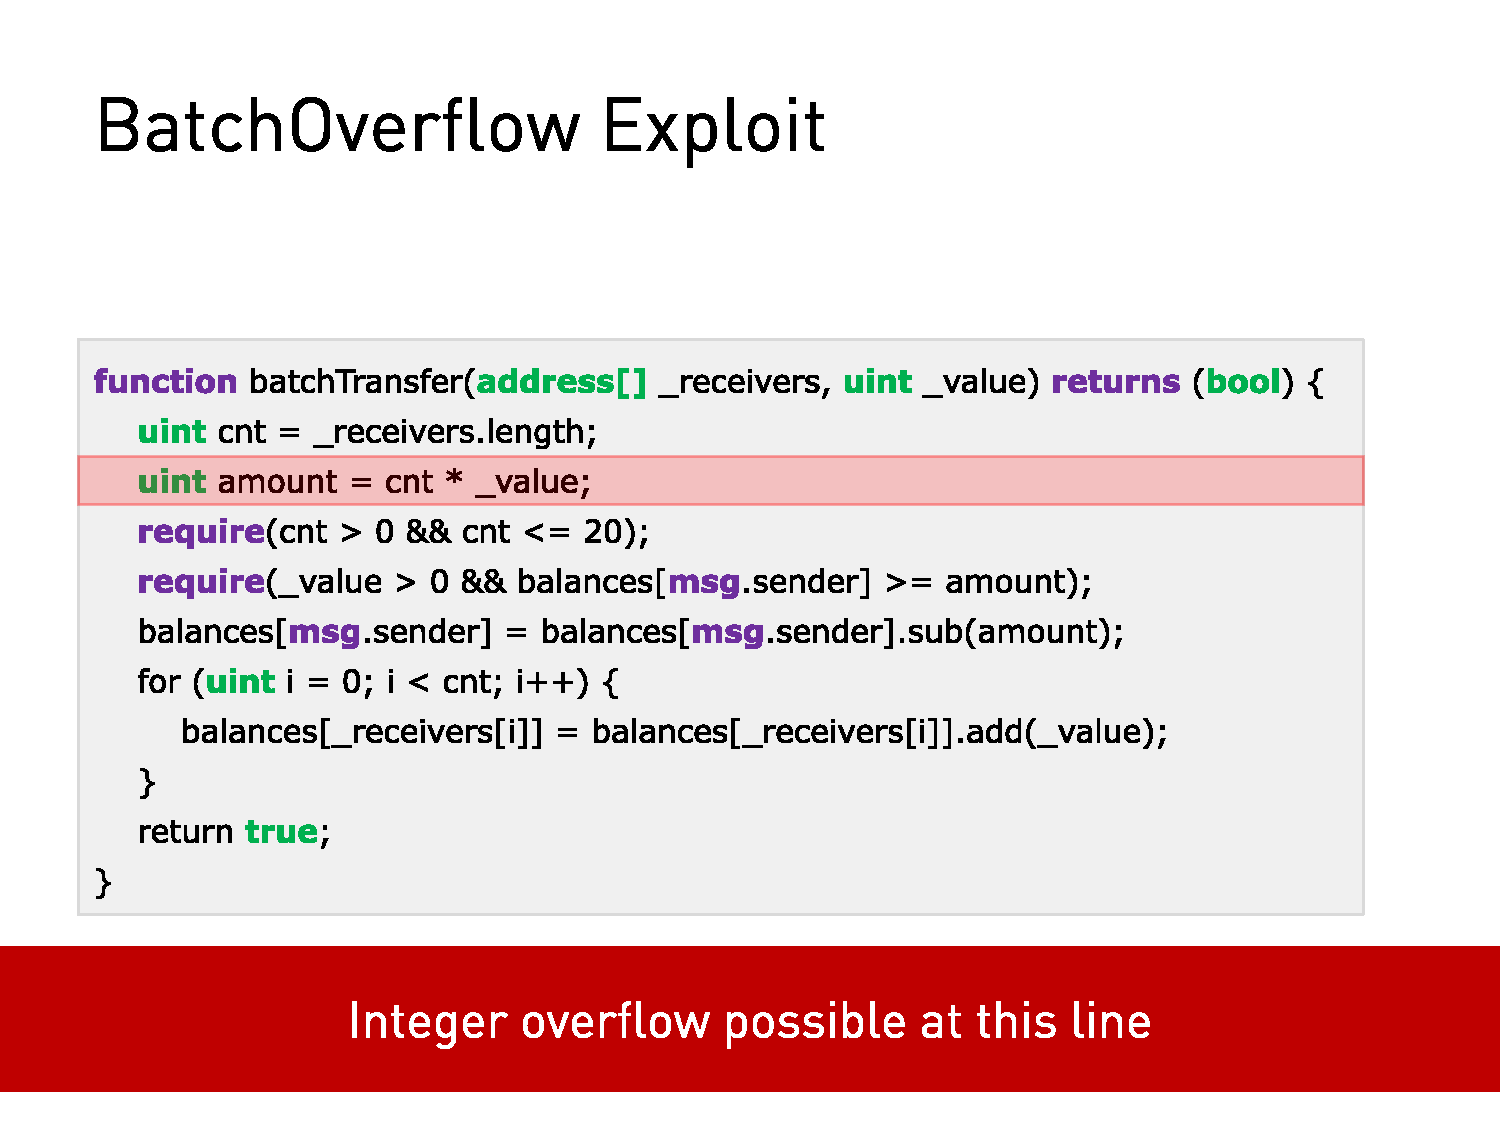
\includegraphics[width=\unitlength,page=1]{Figures/L3_overflow_exploit.pdf}}%
  \end{picture}%
\endgroup%
    
\end{minipage}

\subsection{Semantics and Security Properties}
\begin{itemize}
    \item \textbf{Ethereum virtual machine (EVM) state:} \textcolor{blue}{$\sigma = (S,M,Q,B)$}
    \begin{itemize}
        \item \textcolor{orange}{Storage [S]:} Persistent, inital storage is defined by the constructor.
        \item \textcolor{orange}{Memory [M]:} Not-persistent, re-initialized before  executing a transaction.
        \item \textcolor{orange}{Stack [Q]:} Each element is 256 bits.
        \item \textcolor{orange}{Block information [B]:} Number, timestamp, etc. Fixed for a given transaction.
    \end{itemize}{}
    \item \textbf{Transaction: } \textcolor{blue}{$T = (\texttt{caller}, \texttt{func}, \texttt{args})$}
    \item \textbf{Correctness of smart contracts:} \textcolor{blue}{$\texttt{SmartContract} \implies \texttt{Func/Sec
    Properties}$} 
    \begin{itemize}
        \item Check formal properties for all states.
    \end{itemize}{}
\end{itemize}{}